% Provenance (never printed): see sources/outline_sources.md (Year 3:
% critical-taper theory; fold-and-thrust belts; exhumation and
% thermochronology). Brief: sources/book5/BRIEFS.md, ch. 10. Curves from
% figdata/bachelor-3/fault_bend.py, critical_taper.py and age_elevation.py.
% Exercise and problem values in the Book 5 scratch calculator calc/ch10.py.
\chapter{Thrust Belts and Orogenic Wedges}\label{ch:b3:orogenic-wedges}

Push a bulldozer into wet sand or snow, and a wedge of material piles up in
front of the blade. It deforms until its surface reaches a certain slope;
from then on it slides forward as a whole and grows at the same shape,
taking in new material at its toe. The outer parts of mountain belts, from
Taiwan to the foothills of the Alps, behave in the same way: they are wedges
of rock scraped off a plate and pushed over a weak base, and their surface
slope and the dip of their base tell how weak that base is and how high the
pressure of the fluids within it. This chapter builds the geometry of thrust
belts, the mechanics of the wedge, and the clocks that measure how fast its
rocks come up to the surface.
% ledger: dsd83:taper

\begin{recall}
Thrusts, vergence and fold geometry are in the Year 1 volume, in its chapter
on faults, folds and fabrics; the Coulomb criterion, Byerlee's law, the
effective stress and the pore-pressure ratio $\lambda = P/\sigma_v$ in its
chapter on stress, strain and rheology; closure temperature and cooling age
in its chapter on radiometric dating methods. The décollement, the
fold-and-thrust belt, thin- and thick-skinned tectonics and the balanced
cross-section are in the Year 2 volume, in its chapter on the anatomy of a
mountain belt; exhumation and its rate in its chapter on P--T--t paths. The
kink construction and the excess area $A = Sh$ of a fold above a detachment
are in \cref{ch:b3:structural-analysis}; the \omterm{def:b3:lithosphere-thermal-models:peclet}{thermal Péclet number} in
\cref{ch:b3:lithosphere-thermal-models}.
\end{recall}

\section{The geometry of thrusts}\label{sec:b3:orogenic-wedges:geometry}

A thrust does not cut through a layered sequence along one straight plane.
It follows a weak layer, a shale or an evaporite, for long distances, then
climbs steeply through the strong layers above to the next weak one. The
staircase it draws controls the folds of the hanging wall.

\begin{definition}[Ramp, flat, duplex, out-of-sequence thrust]\label{def:b3:orogenic-wedges:thrust-geometry}
A \emph{flat (thrust)}\index{flat (thrust)} is a segment of a thrust that runs
parallel to the bedding, usually in a weak layer; a \emph{ramp
(thrust)}\index{ramp (thrust)} is a segment that cuts across the bedding,
typically at 20 to \ang{30}, joining a lower flat to an upper one. A
\emph{duplex (thrust)}\index{duplex (thrust)} is a stack of fault-bounded
slices, the horses, enclosed between a floor thrust below and a roof thrust
above, each horse cut off by a ramp that joins the two. Thrusts usually form
in sequence, each new one in the footwall of the previous one, closer to the
foreland; an \emph{out-of-sequence thrust}\index{out-of-sequence thrust} is
one that forms or slips again behind the active front, cutting older thrusts.
\end{definition}

As the hanging wall moves over a bend in the fault, it must fold to stay in
contact with it: a syncline forms where it enters the ramp and an anticline
where it leaves it.

\begin{definition}[Fault-bend, fault-propagation and detachment folds]\label{def:b3:orogenic-wedges:thrust-folds}
A \emph{fault-bend fold}\index{fault-bend fold} is a fold of the hanging wall
of a thrust produced as it slides over a bend of the fault, a ramp between
two flats. A \emph{fault-propagation fold}\index{fault-propagation fold}
grows above the tip of a thrust that is still propagating upward: the
shortening that the fault no longer carries is taken up by folding in front
of its tip, which gives a steep or overturned forelimb. A \emph{detachment
fold}\index{detachment fold} grows above a flat with no ramp: the shortening
is taken up by folding and by a weak layer, salt or shale, that flows into
its core.
\end{definition}

The figure below builds a \omterm{def:b3:orogenic-wedges:thrust-folds}{fault-bend fold}. Here the hanging wall moves
parallel to the fault segment beneath it and folds at axial surfaces that
bisect each bend, a kinematic model called fault-parallel flow; the classic
model of constant layer thickness and length gives the same flat-topped
anticline with a steeper forelimb, at the cost of a longer construction
(admitted here). Both models are bound by the conservation of area.

\begin{omfigure}
\begin{tikzpicture}
\begin{groupplot}[group style={group size=1 by 2, vertical sep=0.9cm},
  width=0.92\linewidth, axis equal image,
  xmin=0, xmax=12, ymin=-0.6, axis lines=none, clip=true,
  title style={font=\small, at={(0.0,1.0)}, anchor=south west}]
% (a) before slip
\nextgroupplot[title={(a) before slip}, ymax=1.75]
\fill[omLithSand!70] (axis cs:0,0) rectangle (axis cs:12,1.6);
\fill[gray!25] (axis cs:0,-0.6) rectangle (axis cs:12,0);
\draw[black!70] (axis cs:0,0.25) -- (axis cs:12,0.25);
\draw[black!70] (axis cs:0,0.5) -- (axis cs:12,0.5);
\draw[black!70] (axis cs:0,0.75) -- (axis cs:12,0.75);
\draw[black!70] (axis cs:0,1.0) -- (axis cs:12,1.0);
\draw[black!70] (axis cs:0,1.3) -- (axis cs:12,1.3);
\draw[black!70] (axis cs:0,1.6) -- (axis cs:12,1.6);
\draw[black!70] (axis cs:0,-0.3) -- (axis cs:12,-0.3);
\addplot[very thick, red!70!black] table[x=x, y=y] {figdata/out/bachelor-3-fault_bend-fault.dat};
\node[font=\scriptsize, fill=omLithSand!70, inner sep=1pt] at (axis cs:2,0.125) {lower flat};
\node[font=\scriptsize, fill=omLithSand!70, inner sep=1pt, rotate=30] at (axis cs:4.55,0.62) {ramp};
\node[font=\scriptsize, fill=omLithSand!70, inner sep=1pt] at (axis cs:9,0.875) {upper flat};
% (b) after a slip of 2.5 units
\nextgroupplot[title={(b) after slip: a fault-bend fold}, ymax=2.75]
\fill[gray!25] (axis cs:0,-0.6) rectangle (axis cs:12,0) -- cycle;
\addplot[name path=fault, draw=none] table[x=x, y=y] {figdata/out/bachelor-3-fault_bend-fault.dat};
\addplot[name path=top, draw=none] table[x=x, y=y] {figdata/out/bachelor-3-fault_bend-bed6.dat};
\addplot[name path=base, draw=none] coordinates {(0,-0.6) (12,-0.6)};
\addplot[omLithSand!70] fill between[of=fault and top];
\addplot[gray!25] fill between[of=base and fault];
\addplot[black!70] table[x=x, y=y] {figdata/out/bachelor-3-fault_bend-bed1.dat};
\addplot[black!70] table[x=x, y=y] {figdata/out/bachelor-3-fault_bend-bed2.dat};
\addplot[black!70] table[x=x, y=y] {figdata/out/bachelor-3-fault_bend-bed3.dat};
\addplot[black!70] table[x=x, y=y] {figdata/out/bachelor-3-fault_bend-bed4.dat};
\addplot[black!70] table[x=x, y=y] {figdata/out/bachelor-3-fault_bend-bed5.dat};
\addplot[black!70] table[x=x, y=y] {figdata/out/bachelor-3-fault_bend-bed6.dat};
\draw[black!70] (axis cs:4.4330,0.25) -- (axis cs:12,0.25);
\draw[black!70] (axis cs:4.8660,0.5) -- (axis cs:12,0.5);
\draw[black!70] (axis cs:5.2990,0.75) -- (axis cs:12,0.75);
\draw[black!70] (axis cs:0,-0.3) -- (axis cs:12,-0.3);
\addplot[very thick, red!70!black] table[x=x, y=y] {figdata/out/bachelor-3-fault_bend-fault.dat};
\draw[densely dashed, black!60] (axis cs:0,1.6) -- (axis cs:12,1.6);
\node[font=\scriptsize, anchor=south] at (axis cs:2.2,1.65) {regional};
\node[font=\scriptsize, anchor=west] at (axis cs:8.6,2.25) {excess area $A = Sr$};
\draw[black!70] (axis cs:8.6,2.25) -- (axis cs:6.6,2.0);
\node[font=\scriptsize, fill=gray!25, inner sep=1pt] at (axis cs:10.6,0.625) {footwall};
\end{groupplot}
\end{tikzpicture}

\par\smallskip{\small (a) A thrust with a lower flat, a ramp dipping
\ang{30} and an upper flat, before slip (schematic, vertical and horizontal
scales equal). (b) The same after a slip of 2.5 times the ramp height,
computed by fault-parallel flow: a syncline at the foot of the ramp, a back
limb parallel to the ramp, a flat crest lifted by the ramp height $r$, a
forelimb, and an excess area $Sr$ above the regional level of every bed above
the upper flat.}\label{fig:b3:orogenic-wedges:thrusts}
\end{omfigure}


\begin{proposition}[Excess area of a fault-bend fold]\label{prop:b3:orogenic-wedges:fault-bend-area}
Let a thrust carry its hanging wall up a ramp of height $r$ from a lower flat
to an upper flat, with the slip $S$ on the lower flat. For any bed of the
hanging wall that lies above the upper flat, the area enclosed between the
folded bed and its original level is $A = Sr$, the same for every such bed.
\end{proposition}

\begin{proof}
Rock is neither created nor destroyed, and its volume is kept. Take a section
parallel to the slip, bounded by two vertical lines far behind and far in
front of the ramp. Through the rear line, the hanging wall between the lower
flat and a bed at the height $y_0$ above it has moved in by $S$: the area
$Sy_0$ has entered. Through the front line, the rock between the upper flat
and the same bed, of thickness $y_0 - r$, has moved out by the slip on the
upper flat, also $S$ when the rock keeps its area: the area $S(y_0 - r)$
has left. The difference, $Sr$, has stayed between the two lines, and lifts
the bed above its original level.
\end{proof}

The excess area of a \omterm{def:b3:orogenic-wedges:thrust-folds}{fault-bend fold} measures the slip times the height of
the ramp, not times the depth to the décollement, as it would for a
\omterm{def:b3:orogenic-wedges:thrust-folds}{detachment fold} (\cref{ch:b3:structural-analysis}). The two kinds of fold
must be told apart before an area is turned into shortening.


A duplex (the figure below) grows when the thrust, instead of carrying its hanging wall ever
farther along the same ramp, abandons it and cuts a new ramp in its footwall,
ahead of the old one. The slice between the old and the new ramp becomes a
horse, carried up the new ramp and stacked beneath the roof; the next ramp
forms ahead again. Each horse is shortened from its original length to the
length it now occupies along the floor, and the shortening of the duplex is
the sum over its horses. \omterm{def:b3:orogenic-wedges:thrust-geometry}{Out-of-sequence thrusts} cut this order: they form
when the wedge behind the front must thicken, a case the mechanics of the
next section predicts.

\begin{omfigure}
\begin{tikzpicture}
\begin{axis}[width=0.92\linewidth, axis equal image, xmin=0, xmax=12, ymin=-0.6, ymax=1.95,
  axis lines=none, clip=true]
\fill[gray!25] (axis cs:0,-0.6) rectangle (axis cs:12,0);
\fill[omLithSand!70] (axis cs:0,0) -- (axis cs:1.0,0) -- (axis cs:2.35,1.15) -- (axis cs:12,1.15) -- (axis cs:12,1.85) -- (axis cs:2.35,1.85) -- (axis cs:1.0,0.7) -- (axis cs:0,0.7) -- cycle;
\draw[black!70] (axis cs:0,0.35) -- (axis cs:1.0,0.35) -- (axis cs:2.35,1.5) -- (axis cs:12,1.5);
\draw[black!70] (axis cs:0,0.7) -- (axis cs:1.0,0.7) -- (axis cs:2.35,1.85) -- (axis cs:12,1.85);
\fill[omLithShale!60] (axis cs:8.2,0) -- (axis cs:12,0) -- (axis cs:12,1.15) -- (axis cs:9.55,1.15) -- cycle;
\draw[black!70] (axis cs:8.646,0.38) -- (axis cs:12,0.38);
\draw[black!70] (axis cs:9.104,0.77) -- (axis cs:12,0.77);
\fill[omLithLime] (axis cs:1.0,0) -- (axis cs:2.80,0) -- (axis cs:4.15,1.15) -- (axis cs:2.35,1.15) -- cycle;
\draw[black!70] (axis cs:1.45,0) -- (axis cs:2.80,1.15);
\draw[black!70] (axis cs:1.90,0) -- (axis cs:3.25,1.15);
\draw[black!70] (axis cs:2.35,0) -- (axis cs:3.70,1.15);
\fill[omLithShale] (axis cs:2.8,0) -- (axis cs:4.60,0) -- (axis cs:5.95,1.15) -- (axis cs:4.15,1.15) -- cycle;
\draw[black!70] (axis cs:3.25,0) -- (axis cs:4.60,1.15);
\draw[black!70] (axis cs:3.70,0) -- (axis cs:5.05,1.15);
\draw[black!70] (axis cs:4.15,0) -- (axis cs:5.50,1.15);
\fill[omLithLime] (axis cs:4.6,0) -- (axis cs:6.40,0) -- (axis cs:7.75,1.15) -- (axis cs:5.95,1.15) -- cycle;
\draw[black!70] (axis cs:5.05,0) -- (axis cs:6.40,1.15);
\draw[black!70] (axis cs:5.50,0) -- (axis cs:6.85,1.15);
\draw[black!70] (axis cs:5.95,0) -- (axis cs:7.30,1.15);
\fill[omLithShale] (axis cs:6.4,0) -- (axis cs:8.20,0) -- (axis cs:9.55,1.15) -- (axis cs:7.75,1.15) -- cycle;
\draw[black!70] (axis cs:6.85,0) -- (axis cs:8.20,1.15);
\draw[black!70] (axis cs:7.30,0) -- (axis cs:8.65,1.15);
\draw[black!70] (axis cs:7.75,0) -- (axis cs:9.10,1.15);
\draw[thick, red!70!black] (axis cs:1.0,0) -- (axis cs:2.35,1.15);
\draw[thick, red!70!black] (axis cs:2.8,0) -- (axis cs:4.15,1.15);
\draw[thick, red!70!black] (axis cs:4.6,0) -- (axis cs:5.95,1.15);
\draw[thick, red!70!black] (axis cs:6.4,0) -- (axis cs:7.75,1.15);
\draw[thick, red!70!black] (axis cs:8.2,0) -- (axis cs:9.55,1.15);
\draw[very thick, red!70!black] (axis cs:0,0) -- (axis cs:12,0);
\draw[very thick, red!70!black] (axis cs:2.35,1.15) -- (axis cs:12,1.15);
\node[font=\scriptsize, anchor=north west] at (axis cs:0.1,-0.04) {floor thrust};
\node[font=\scriptsize, anchor=south west] at (axis cs:7.0,1.17) {roof thrust};
\node[font=\scriptsize, anchor=north] at (axis cs:5.6,-0.12) {horse};
\draw[black!70] (axis cs:5.6,-0.15) -- (axis cs:5.5,0.45);
\draw[->, thick] (axis cs:0.15,0.52) -- (axis cs:0.95,0.52);
\end{axis}
\end{tikzpicture}

\par\smallskip{\small A duplex (schematic): four horses (blue and green) cut
off by ramps between a floor and a roof thrust, ahead of them the footwall not
yet cut, the arrow giving the sense of transport; the cover above the roof is
folded over the stack.}\label{fig:b3:orogenic-wedges:duplex}
\end{omfigure}


\section{The critical taper}\label{sec:b3:orogenic-wedges:taper}

A fold-and-thrust belt in cross-section is a wedge: thin at its front, where
the décollement reaches the surface, and thickening towards the hinterland.
Its upper surface slopes towards the foreland at the angle $\alpha$; its
base, the décollement, dips towards the hinterland at the angle $\beta$. The
taper of the wedge is the angle between them, $\alpha + \beta$.

\begin{definition}[Critical taper]\label{def:b3:orogenic-wedges:critical-taper}
The \emph{critical taper}\index{critical taper} of a wedge pushed from behind
over a base is the taper at which the wedge is everywhere on the verge of
failure, inside and along its base, under horizontal compression. A wedge at
its critical taper slides over its base without deforming internally; a
wedge below it (subcritical) deforms and thickens until it reaches it; a
wedge above it (supercritical) slides without deforming.
\end{definition}
% ledger: dsd83:taper

\begin{omfigure}
\begin{tikzpicture}[>=stealth, x=1cm, y=1cm]
\fill[omLithSand!70] (0,0) -- (10,-1.05) -- (10,1.4) -- cycle;
\fill[gray!25] (0,0) -- (10,-1.05) -- (10,-1.6) -- (-0.8,-1.6) -- (-0.8,0) -- cycle;
\draw[thick] (-0.8,0) -- (0,0) -- (10,1.4);
\draw[very thick, red!70!black] (0,0) -- (10,-1.05);
\fill[gray!60] (10,-1.6) rectangle (10.6,1.9);
\node[font=\scriptsize, rotate=90] at (10.3,0.15) {backstop};
\draw[dashed] (0,0) -- (2.6,0);
\draw (2.2,0) arc[start angle=0, end angle=8, radius=2.2];
\node[font=\small] at (2.45,0.2) {$\alpha$};
\draw (2.2,0) arc[start angle=0, end angle=-6, radius=2.2];
\node[font=\small] at (2.45,-0.2) {$\beta$};
% slice
\draw[thick, omDef] (5.5,-0.5775) -- (5.5,0.77);
\draw[thick, omDef] (6.5,-0.6825) -- (6.5,0.91);
\draw[->, thick, omDef] (4.5,0.05) -- (5.45,0.05);
\node[font=\scriptsize, anchor=east] at (4.5,0.05) {$F(x)$};
\draw[<-, thick, omDef] (6.55,0.1) -- (7.6,0.1);
\node[font=\scriptsize, anchor=west] at (7.6,0.1) {$F(x + \mathrm dx)$};
\draw[->, thick, omProp] (6.0,-0.63) -- (6.75,-0.71);
\node[font=\scriptsize, anchor=north] at (6.4,-0.75) {$\tau_b$};
\draw[->, thick, omProp] (6.0,-0.63) -- (6.1,0.0);
\node[font=\scriptsize, anchor=east] at (6.02,-0.22) {$\sigma_n$};
\node[font=\scriptsize] at (6.0,1.2) {slice $\mathrm dx$};
\draw[->, thick] (1.8,-1.25) -- (0.6,-1.25);
\node[font=\scriptsize, anchor=west] at (1.85,-1.25) {transport};
\node[font=\scriptsize, anchor=west] at (0.2,-0.42) {décollement};
\node[font=\scriptsize] at (8.9,-0.45) {wedge};
\draw[->] (0.1,0.5) -- (0.4,0.5); \node[font=\scriptsize, anchor=east] at (0.1,0.5) {$x$};
\end{tikzpicture}

\par\smallskip{\small A wedge of surface slope $\alpha$ resting on a
décollement of dip $\beta$ and pushed from behind; $x$ is measured from the
toe towards the hinterland. On a vertical slice, the push $F(x + \mathrm dx)$
from behind exceeds the push $F(x)$ from the front by what the base takes:
its friction $\tau_b$ and the horizontal part of its normal stress $\sigma_n$,
which leans towards the hinterland on a base dipping that way (schematic,
angles exaggerated).}\label{fig:b3:orogenic-wedges:wedge}
\end{omfigure}

\begin{theorem}[Critical-taper equation]\label{thm:b3:orogenic-wedges:critical-taper}
Consider a subaerial wedge of uniform density $\rho$ made of cohesionless
Coulomb material of internal friction $\mu = \tan\phi$, with the pore-pressure
ratio $\lambda$, on a base of friction $\mu_b$ and pore-pressure ratio
$\lambda_b$. If $\alpha$ and $\beta$ are small and $\sigma_1$ is horizontal,
the \emph{critical-taper equation}\index{critical-taper equation} is
\[
  \alpha + \beta = \frac{\beta + \mu_b(1 - \lambda_b)}{1 + K(1 - \lambda)},
  \qquad K = \frac{2\sin\phi}{1 - \sin\phi},
\]
with the angles in radians.
\end{theorem}

\begin{proof}
Let $z$ be the depth below the surface. With small slopes, the vertical
stress is the weight of the rock above, $\sigma_{zz} = \rho g z$, and the pore
pressure is $\lambda\rho g z$, so that the effective vertical stress is
$(1 - \lambda)\rho g z$. Everywhere at failure with $\sigma_1$ horizontal,
the Coulomb criterion for a cohesionless material gives the ratio of the
effective principal stresses $\sigma'_1/\sigma'_3 = (1 + \sin\phi)/(1 -
\sin\phi) = 1 + K$, hence the total horizontal stress
\[
  \sigma_{xx} = (1 + K)(1 - \lambda)\rho g z + \lambda\rho g z
  = \bigl(1 + K(1 - \lambda)\bigr)\rho g z .
\]
At the distance $x$ from the toe the wedge has the thickness $H = (\alpha +
\beta)x$, and the horizontal force per unit length of the belt on a vertical
section is $F = \int_0^H \sigma_{xx}\,\mathrm dz = \bigl(1 + K(1 -
\lambda)\bigr)\rho g H^2/2$. On the slice between $x$ and $x + \mathrm dx$
(the figure above), the surface carries no stress and the push from behind
exceeds the push from the front by $(\mathrm dF/\mathrm dx)\,\mathrm dx$.
The base holds the slice back in two ways: the friction $\mu_b(1 -
\lambda_b)\rho g H$ per unit length, and its normal stress $\rho g H$, which
is perpendicular to a base dipping $\beta$ towards the hinterland and so
leans that way by $\beta$, giving the horizontal part $\beta\rho g H$.
Equilibrium of the slice requires
\[
  \bigl(1 + K(1 - \lambda)\bigr)\rho g H(\alpha + \beta)
  = \bigl(\beta + \mu_b(1 - \lambda_b)\bigr)\rho g H ,
\]
which is the equation. Since $H$ cancels, a wedge at failure keeps the same
taper as it grows.
\end{proof}

The equation says, first, that the taper is set by the ratio of the strength
of the base, in the numerator, to the strength of the wedge, in the
denominator: a weak base gives a thin wedge, a strong base a thick one.
Second, the surface slope falls as the base dips more steeply. Third, fluid
pressure lowers the taper: raising $\lambda = \lambda_b$ takes from the
strength of the base more, in proportion, than from the strength of the
wedge. The figure below shows the critical surface slope for the friction
coefficients fitted in western Taiwan. Points below each line are subcritical
wedges, which thicken; points above are supercritical, which slide.
% ledger: dsd83:taper

\begin{omfigure}
\begin{tikzpicture}
\begin{axis}[omrecord, width=0.8\linewidth, height=0.5\linewidth,
  xlabel={basal dip $\beta$ (\unit{\degree})}, ylabel={surface slope $\alpha$ (\unit{\degree})},
  xmin=0, xmax=15, ymin=0, ymax=12, legend style={font=\scriptsize, at={(0.98,0.98)},
  anchor=north east, legend cell align=left}]
% computed in figdata/bachelor-3/critical_taper.py
\addplot[name path=t3, draw=none, forget plot] table[x=beta, y=t3] {figdata/out/bachelor-3-critical_taper-bands.dat};
\addplot[name path=t4, draw=none, forget plot] table[x=beta, y=t4] {figdata/out/bachelor-3-critical_taper-bands.dat};
\addplot[name path=t12, draw=none, forget plot] table[x=beta, y=t12] {figdata/out/bachelor-3-critical_taper-bands.dat};
\addplot[name path=t13, draw=none, forget plot] table[x=beta, y=t13] {figdata/out/bachelor-3-critical_taper-bands.dat};
\addplot[omLithEvap, area legend] fill between[of=t3 and t4];
\addlegendentry{taper 3--\ang{4} (Jura)}
\addplot[omLithLime, area legend] fill between[of=t12 and t13];
\addlegendentry{taper 12--\ang{13}}
\addplot[omDef, thick] table[x=beta, y=a040] {figdata/out/bachelor-3-critical_taper-curves.dat};
\addlegendentry{$\lambda = 0.4$}
\addplot[red!70!black, thick, densely dashed] table[x=beta, y=a070] {figdata/out/bachelor-3-critical_taper-curves.dat};
\addlegendentry{$\lambda = 0.7$}
\addplot[black, thick, densely dotted] table[x=beta, y=a090] {figdata/out/bachelor-3-critical_taper-curves.dat};
\addlegendentry{$\lambda = 0.9$}
\node[font=\scriptsize] at (axis cs:2.2,1.1) {subcritical};
\node[font=\scriptsize] at (axis cs:1.6,8.6) {supercritical};
\end{axis}
\end{tikzpicture}

\par\smallskip{\small Critical surface slope against basal dip for the
friction coefficients of western Taiwan, $\mu = 1.03$ inside and $\mu_b =
0.85$ on the base, for three pore-pressure ratios $\lambda = \lambda_b$;
``subcritical'' and ``supercritical'' refer to the $\lambda = 0.7$ line. The
shaded bands are the tapers of the Jura thrust wedge, 3 to \ang{4}, and of the
wedge to its south, 12 to \ang{13}.}\label{fig:b3:orogenic-wedges:taper}
\end{omfigure}
% ledger: dsd83:taper, deville21:jura

A wedge is not a static object: material is added to it and removed from it,
and each change pushes it off its \omterm{def:b3:orogenic-wedges:critical-taper}{critical taper}.

\begin{definition}[Frontal accretion, tectonic underplating]\label{def:b3:orogenic-wedges:accretion}
\emph{Frontal accretion}\index{frontal accretion} is the addition of material
to a wedge at its toe, as the décollement propagates into the undeformed
sediments of the foreland and a new thrust slice is cut. \emph{Tectonic
underplating}\index{tectonic underplating} is the addition of material to
the base of the wedge, behind its toe, as slices of the lower plate are
detached and stacked beneath it, often as duplexes.
\end{definition}

\omterm{def:b3:orogenic-wedges:accretion}{Frontal accretion} lengthens the wedge at constant taper. Underplating
thickens its rear and steepens its surface: the wedge becomes supercritical
there and may extend by normal faulting until the taper falls back. Erosion
does the opposite: it lowers the surface slope, the wedge becomes
subcritical, and it thickens by out-of-sequence thrusting behind the front.
Erosion and deformation are thus coupled: a wedge eroded fast keeps its
taper by moving rock upward faster, and the rocks it brings to the surface
are younger in the sense of the next section.

\begin{inthelab}[Sandbox models]
\begin{minipage}[t]{0.55\linewidth}\vspace{0pt}
In an analogue sandbox model, layers of dry sand of different colours are
laid flat in a long glass-sided box. A motor slowly pushes a vertical wall into them,
or pulls a sheet out from beneath them; a camera beside the glass photographs the section at regular
steps. The sand fails along thrusts, grows a wedge that keeps a constant
taper, and develops ramps, duplexes and back-thrusts like those of real
belts. A layer of glass beads or of a silicone putty beneath the sand plays
the part of a weak décollement, and the wedge then grows thinner and wider.
Davis, Suppe and Dahlen found that their experiments with dry sand matched the
critical-taper theory. Correlating the successive photographs gives the
displacement field inside the model.
\end{minipage}\hfill
\begin{minipage}[t]{0.42\linewidth}\vspace{0pt}
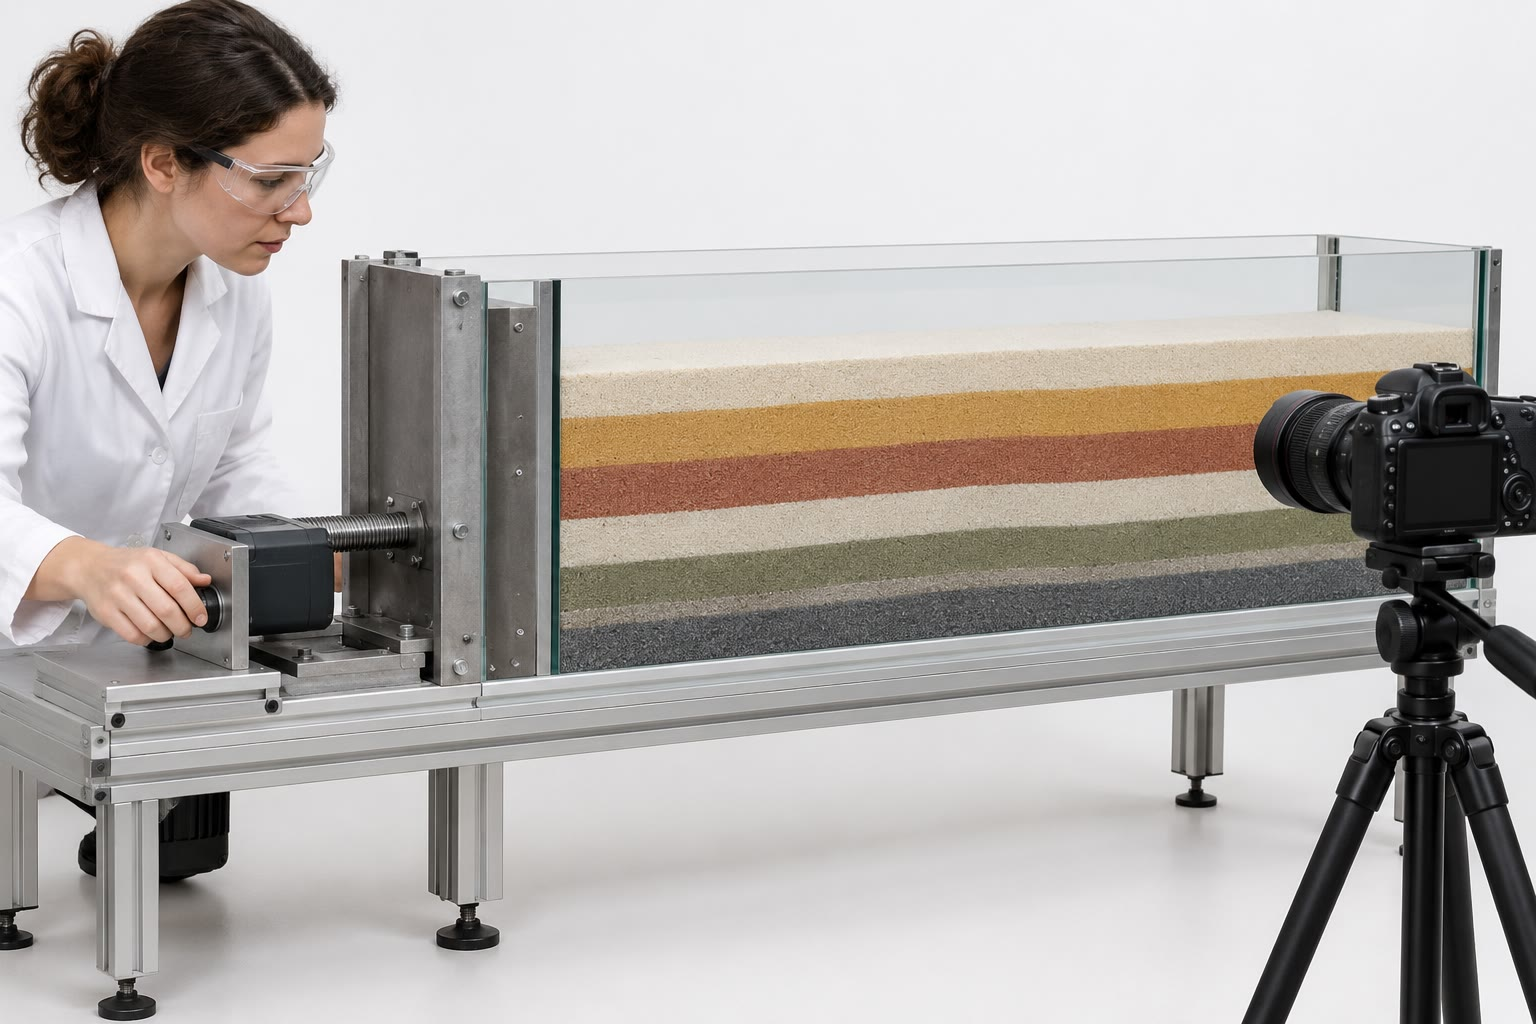
\includegraphics[width=\linewidth]{images/book5/ai/b3-sandbox-lab.jpg}

{\scriptsize A sandbox model before shortening: coloured sand layers in a
glass-sided box, a motor-driven wall at the left, a camera on a tripod
(AI-generated illustration).}
\end{minipage}
\end{inthelab}
% ledger: dsd83:taper

\section{Real wedges}\label{sec:b3:orogenic-wedges:real}

In the active fold-and-thrust belt of western Taiwan, the surface slope, the
dip of the décollement and the pore pressures are all known, from topography,
seismic sections and wells. Davis, Suppe and Dahlen used them to solve the
\omterm{thm:b3:orogenic-wedges:critical-taper}{critical-taper equation} for the strength of the wedge and found $\mu = 1.03$
inside and $\mu_b = 0.85$ on the base: Byerlee's friction on the base, and a
wedge stronger than its own faults, because they are not all oriented to slip
easily. With these two coefficients they turned the observed tapers of other
active wedges, on land and under the sea, into pore-pressure ratios, and found
them everywhere above hydrostatic, in line with drilling. They also found
where the theory stops: the taper drops abruptly where wedges grow thicker
than about \qty{15}{km}, the depth at which quartz-rich rocks become plastic
for common geotherms, and the base no longer obeys a frictional law.
% ledger: dsd83:taper

At the front of the western Alps, the Jura is a thrust wedge with a narrow
angle of only 3 to \ang{4}. Its décollement lies mostly in halite-bearing
layers of Triassic age, and the fluids there are not overpressured: the
weakness of salt alone explains the narrow taper. South of the Jura, where the
Triassic layers hold no halite, the same front has a taper of 12 to
\ang{13}, with stacks of thrust slices, although fluid pressures measured
there are high. In the Central Alps, critical-taper analysis of the surface
slope gives a basal strength $\mu_b(1 - \lambda_b)$ (with a small cohesion
term) below 0.1, and even 0.05 in evaporites and shales near the front,
increasing towards the hinterland, with pore-pressure ratios above 0.54. The
base of a wedge is often far weaker than Byerlee's law would make it, by its
rock type and by its fluids.
% ledger: deville21:jura, vonhagke14:alps

\section{Flux through a wedge}\label{sec:b3:orogenic-wedges:flux}

A wedge at its \omterm{def:b3:orogenic-wedges:critical-taper}{critical taper} grows by accretion, at fixed shape: its length
and height increase together. Erosion removes rock from its surface. When the
two balance, the wedge keeps its size, and rock flows through it.

\begin{proposition}[Steady-state flux balance]\label{prop:b3:orogenic-wedges:flux}
A wedge of width $W$ along the transport direction receives, per unit length
of the belt, the accretionary flux $F_a = v h$, where $v$ is the convergence
rate and $h$ the thickness of the incoming layer above the décollement. It
loses the erosional flux $F_e = \bar e W$, where $\bar e$ is the mean erosion
rate over its surface. Its cross-sectional area changes at the rate $F_a -
F_e$; at steady state, $\bar e = vh/W$.
\end{proposition}

\begin{proof}
In unit time, a length $v$ of the incoming layer, of thickness $h$, passes
into the wedge across its toe, and the thickness $e(x)$ is removed at each
point of its surface; the area is conserved, so the area of the section
changes by $vh - \int_0^W e\,\mathrm dx = F_a - F_e$. At steady state the
change is zero.
\end{proof}

With $v = \qty{10}{mm/yr}$, $h = \qty{4}{km}$ and $W = \qty{60}{km}$, the
erosion rate needed for steady state is $\qty{0.67}{mm/yr}$. Exhumation in the
sense of the Year 2 volume is the removal of the rock above a given rock:
at steady state, rocks reach the surface at the rate at which erosion lowers
it, and the wedge brings them up from depths where they were hot. Measuring
how fast requires a clock that starts at a known temperature.

\section{Thermochronology}\label{sec:b3:orogenic-wedges:thermochronology}

\begin{definition}[Thermochronology, thermochronometer]\label{def:b3:orogenic-wedges:thermochronology}
\emph{Thermochronology}\index{thermochronology} is the use of radiometric
cooling ages to date the time at which a rock passed through a given
temperature, and so to reconstruct its thermal history. A
\emph{thermochronometer}\index{thermochronometer} is a pair of a mineral and
a dating method with its closure temperature: for instance apatite with the
(U--Th)/He method, or zircon with fission tracks.
\end{definition}

The table below orders the main \omterm{def:b3:orogenic-wedges:thermochronology}{thermochronometers} by closure temperature;
the depths assume a mean surface temperature of \qty{10}{\celsius} and a
uniform gradient of \qty{30}{\celsius/km}. A rock that cools as it is
exhumed passes them in turn, and its ages grow from the low-temperature
methods to the high-temperature ones. The physics of fission tracks and of
helium diffusion, which sets these temperatures, is in
\cref{ch:b3:advanced-geochronology}.
\begin{center}
\small
% ledger: sueoka19:closure
\begin{tabular}{lcc}
\hline
\omterm{def:b3:orogenic-wedges:thermochronology}{thermochronometer} & closure temperature (\unit{\celsius}) & depth (\unit{km}) \\
\hline
apatite (U--Th)/He & 50--80 & 1.3--2.3 \\
apatite fission track & 90--120 & 2.7--3.7 \\
zircon (U--Th)/He & 160--200 & 5.0--6.3 \\
zircon fission track & about 280 & 9 \\
\textsuperscript{40}Ar/\textsuperscript{39}Ar on biotite & 350--400 & 11--13 \\
\textsuperscript{40}Ar/\textsuperscript{39}Ar on muscovite & about 425 & 14 \\
U--Pb on zircon & above 900 & --- \\
\hline
\end{tabular}
\end{center}

These depths are only a first guess, because erosion changes the geotherm.

\begin{proposition}[Steady-state geotherm with erosion]\label{prop:b3:orogenic-wedges:geotherm}
Let rock rise at the constant speed $v$ through a layer of thickness $L$ whose
surface ($z = 0$) is held at $T_s$ and base at $T_L$, with no heat
production. The steady temperature is
\[
  T(z) = T_s + (T_L - T_s)\,\frac{1 - e^{-\mathrm{Pe}\,z/L}}{1 - e^{-\mathrm{Pe}}},
  \qquad \mathrm{Pe} = \frac{vL}{\kappa},
\]
and the gradient at the surface is $\mathrm{Pe}/(1 - e^{-\mathrm{Pe}})$ times
the conductive gradient $(T_L - T_s)/L$.
\end{proposition}

\begin{proof}
A rock particle at the depth $z$ moves upward, toward smaller $z$: the
temperature it carries changes as $\partial T/\partial t - v\,\partial
T/\partial z$, and the diffusion equation becomes $\partial T/\partial t - v
T' = \kappa T''$. At steady state, $T'' = -(v/\kappa)T'$, so $T' = C
e^{-vz/\kappa}$ and $T = T_s + C(\kappa/v)(1 - e^{-vz/\kappa})$, which meets
$T(0) = T_s$. Setting $T(L) = T_L$ fixes $C$ and gives the formula. At $z =
0$, $T' = (T_L - T_s)(\mathrm{Pe}/L)/(1 - e^{-\mathrm{Pe}})$.
\end{proof}

For $\mathrm{Pe} \ll 1$ the factor tends to 1: conduction wins and the
geotherm stays straight. For $v = \qty{1}{mm/yr}$ across \qty{30}{km}, with
$\kappa = \qty{e-6}{m^2/s}$, $\mathrm{Pe} = 0.95$ and the surface gradient
rises from 30 to \qty{46}{\celsius/km}: the isotherms crowd towards the
surface and every \omterm{def:b3:orogenic-wedges:thermochronology}{thermochronometer} closes shallower.
% ledger: england:kelvin, earle:settings

\begin{definition}[Age--elevation relationship]\label{def:b3:orogenic-wedges:age-elevation}
The \emph{age--elevation relationship}\index{age--elevation relationship} of a
\omterm{def:b3:orogenic-wedges:thermochronology}{thermochronometer} is the plot of the cooling ages of samples collected over a
range of elevations, usually along a steep slope or a vertical profile,
against their elevations.
\end{definition}

\begin{proposition}[Slope of the age--elevation relationship]\label{prop:b3:orogenic-wedges:age-elevation}
Let rocks rise vertically at the constant speed $v$ under a steady
topography, and let the closure isotherm lie at the elevation $e(x) = e_0 +
f\,h(x)$, where $h(x)$ is the surface elevation and $0 \le f < 1$. A sample
collected at the surface at the elevation $h$ has the age $t = (h - e)/v$,
and the \omterm{def:b3:orogenic-wedges:age-elevation}{age--elevation relationship} is a straight line of slope
\[
  \frac{\mathrm dh}{\mathrm dt} = \frac{v}{1 - f}.
\]
With a flat isotherm, $f = 0$ and the slope is the exhumation rate.
\end{proposition}

\begin{proof}
The rock now at the surface at $x$ crossed the closure isotherm directly
below, at the elevation $e(x)$, and has risen $h - e$ since, at the speed $v$:
$t = (h - e_0 - fh)/v = ((1 - f)h - e_0)/v$. Hence $\mathrm dt/\mathrm dh =
(1 - f)/v$.
\end{proof}

\begin{omfigure}
\begin{tikzpicture}
\begin{groupplot}[group style={group size=2 by 1, horizontal sep=1.7cm},
  omrecord, width=0.47\linewidth, height=0.45\linewidth, title style={font=\small},
  legend style={font=\scriptsize, legend cell align=left}]
\nextgroupplot[title={(a) age--elevation}, xlabel={apatite (U--Th)/He age (\unit{Myr})},
  ylabel={elevation above the mean (\unit{km})}, xmode=log, xmin=0.1, xmax=10,
  log ticks with fixed point, xtick={0.1,0.2,0.5,1,2,5,10}, ymin=-1, ymax=1]
% computed in figdata/bachelor-3/age_elevation.py
\addplot[black, thick, densely dotted] table[x=a30, y=h] {figdata/out/bachelor-3-age_elevation-ages.dat};
\addplot[red!70!black, thick, densely dashed] table[x=a10, y=h] {figdata/out/bachelor-3-age_elevation-ages.dat};
\addplot[omDef, thick] table[x=a03, y=h] {figdata/out/bachelor-3-age_elevation-ages.dat};
\nextgroupplot[title={(b) the closure isotherm}, xlabel={distance (\unit{km})},
  ylabel={elevation above the mean (\unit{km})}, xmin=0, xmax=40, ymin=-3.3, ymax=1.2,
  legend style={at={(0.5,0.03)}, anchor=south, legend columns=2}]
\addplot[black!70, very thick] table[x=x, y=h] {figdata/out/bachelor-3-age_elevation-iso.dat};
\addlegendentry{surface}
\addplot[black, thick, densely dotted] table[x=x, y=e30] {figdata/out/bachelor-3-age_elevation-iso.dat};
\addlegendentry{\qty{3}{mm/yr}}
\addplot[red!70!black, thick, densely dashed] table[x=x, y=e10] {figdata/out/bachelor-3-age_elevation-iso.dat};
\addlegendentry{\qty{1}{mm/yr}}
\addplot[omDef, thick] table[x=x, y=e03] {figdata/out/bachelor-3-age_elevation-iso.dat};
\addlegendentry{\qty{0.3}{mm/yr}}
\end{groupplot}
\end{tikzpicture}

\par\smallskip{\small Steady exhumation under a sinusoidal relief of
wavelength \qty{20}{km} and amplitude \qty{1}{km}, for three rates,
line styles as in the legend of (b) (first-order model; layer \qty{30}{km} thick, surface at \qty{10}{\celsius},
\qty{30}{\celsius/km} without erosion, $\kappa = \qty{e-6}{m^2/s}$, lapse
rate \qty{6.5}{\celsius/km}, closure at \qty{65}{\celsius}). (a) Age against
elevation: the slopes are 0.59, 2.5 and \qty{14}{mm/yr}, not 0.3, 1 and 3.
(b) The \qty{65}{\celsius} isotherm follows the topography more closely the
faster the exhumation, as it rises nearer to the surface.}\label{fig:b3:orogenic-wedges:age-elevation}
\end{omfigure}
% ledger: earle:settings, england:kelvin, ussa76:layers, sueoka19:closure

Isotherms are not flat beneath a relief: the surface is colder on the peaks
than in the valleys, by the atmospheric lapse rate, but much less so than the
rock would be at the same elevation underground, and the shallow isotherms
follow the topography in a subdued way. For a sinusoidal topography of
wavelength $\Lambda$ and a lapse rate $\Gamma$, a first-order solution of the
steady equation gives
\[
  f = \frac{(G_0 - \Gamma)\,e^{-mz_c}}{G(z_c)},\qquad
  m = \frac{v}{2\kappa} + \sqrt{\Bigl(\frac{v}{2\kappa}\Bigr)^2 +
  \Bigl(\frac{2\pi}{\Lambda}\Bigr)^2},
\]
where $z_c$ is the depth of the closure isotherm below the mean surface,
$G_0$ the surface gradient and $G(z_c)$ the gradient at $z_c$ (admitted;
the script tests it). The perturbation dies away with depth over the
distance $1/m$, at most $\Lambda/2\pi$: low-temperature \omterm{def:b3:orogenic-wedges:thermochronology}{thermochronometers},
which close shallow, feel the relief most. The figure above shows the effect
for apatite (U--Th)/He.
% ledger: sueoka19:closure, ussa76:layers

An age--elevation profile measures the exhumation rate only where the
closure isotherm is flat beneath the relief. Elsewhere it overestimates it, by the factor $1/(1 - f)$, which reaches
two or more for apatite (U--Th)/He in a relief of \qty{20}{km} wavelength.
Ages from several \omterm{def:b3:orogenic-wedges:thermochronology}{thermochronometers} on the same samples, and thermal models
of the relief, correct for it.

\section{Exercises}

\begin{exercise}[$\star$]\label{exo:b3:orogenic-wedges:1}
Compute $K$ and the ratio $\sigma'_1/\sigma'_3$ at failure for a wedge with
$\phi = \ang{30}$.
\end{exercise}

\begin{exercise}[$\star$]\label{exo:b3:orogenic-wedges:2}
A sandbox wedge of dry sand ($\lambda = \lambda_b = 0$) has $\mu = 0.6$
inside and $\mu_b = 0.3$ on its base. Compute its critical surface slope on a
horizontal base, then on a base dipping \ang{3}.
\end{exercise}

\begin{exercise}[$\star$]\label{exo:b3:orogenic-wedges:3}
With a surface at \qty{10}{\celsius} and a gradient of \qty{30}{\celsius/km},
check the depths of the table of closure temperatures for apatite
(U--Th)/He, apatite fission track and zircon fission track. Which
\omterm{def:b3:orogenic-wedges:thermochronology}{thermochronometer} would you use to date exhumation from \qty{5}{km}?
\end{exercise}

\begin{exercise}[$\star$]\label{exo:b3:orogenic-wedges:4}
A ramp \qty{2}{km} high dips \ang{30}. Compute its horizontal length and its
length along the dip. By how much is a bed of the hanging wall lifted once it
has crossed the whole ramp, and what slip brings the cut-off of the lowest
bed from the foot of the ramp to the upper flat?
\end{exercise}

\begin{exercise}[$\star\star$]\label{exo:b3:orogenic-wedges:5}
With the Taiwan coefficients, compute the critical surface slope on a base
dipping \ang{6} for $\lambda = \lambda_b = 0.4$ and $0.9$. What does an
increase of the fluid pressure do to a wedge that was at its \omterm{def:b3:orogenic-wedges:critical-taper}{critical taper}?
\end{exercise}

\begin{exercise}[$\star\star$]\label{exo:b3:orogenic-wedges:6}
A \omterm{def:b3:orogenic-wedges:thrust-folds}{fault-bend fold} lies above a ramp \qty{1.5}{km} high; a bed above the upper
flat shows an excess area of \qty{6.0}{km^2}. Compute the slip. A colleague
reads the same fold as a \omterm{def:b3:orogenic-wedges:thrust-folds}{detachment fold}, the bed lying \qty{3.0}{km} above
the décollement. What shortening would he find?
\end{exercise}

\begin{exercise}[$\star\star$]\label{exo:b3:orogenic-wedges:7}
Take $\mu = 0.6$ inside both the Jura wedge (taper \ang{3.5}) and the wedge to
its south (taper \ang{12.5}), a hydrostatic $\lambda = 0.4$ inside both, and a
basal dip of \ang{2} for both. Compute the basal strength $\mu_b(1 -
\lambda_b)$ that each taper requires, and compare it with Byerlee's $0.85$
at hydrostatic pressure. Is the result consistent with the décollement in
halite beneath the Jura?
\end{exercise}

\begin{exercise}[$\star\star$]\label{exo:b3:orogenic-wedges:8}
Rock rises at \qty{1}{mm/yr} through a layer \qty{30}{km} thick, from
\qty{910}{\celsius} at its base to \qty{10}{\celsius} at the surface, with
$\kappa = \qty{e-6}{m^2/s}$. Compute the Péclet number, the surface gradient,
and the depth of the \qty{65}{\celsius} isotherm. Compare with the depth
without erosion.
\end{exercise}

\begin{exercise}[$\star\star$]\label{exo:b3:orogenic-wedges:9}
Two samples from the same slope, at 1200 and \qty{2000}{m}, have apatite
(U--Th)/He ages of 3.4 and \qty{4.6}{Myr}. Compute the apparent exhumation
rate. A thermal model of the relief gives $f = 0.5$: what is the true rate?
\end{exercise}

\begin{exercise}[$\star\star\star$]\label{exo:b3:orogenic-wedges:10}
Show that, for $\lambda = \lambda_b$, the critical surface slope vanishes at a
basal dip $\beta^* = \mu_b/K$ that does not depend on $\lambda$. Compute it for
Taiwan. What happens to a wedge whose base dips more steeply?
\end{exercise}

\begin{exercise}[$\star\star\star$]\label{exo:b3:orogenic-wedges:11}
Show that, for a very long wavelength and a very slow exhumation, $f$ tends to
$1 - \Gamma/G$, where $G$ is the uniform gradient; evaluate it for $G =
\qty{30}{\celsius/km}$ and $\Gamma = \qty{6.5}{\celsius/km}$. What is then the
slope of the \omterm{def:b3:orogenic-wedges:age-elevation}{age--elevation relationship}? For $v = \qty{1}{mm/yr}$ and the
values of exercise~8 ($z_c = \qty{1.21}{km}$, $G_0 = \qty{46.5}{\celsius/km}$,
$G(z_c) = \qty{44.7}{\celsius/km}$), compute $f$ for wavelengths of 5 and
\qty{20}{km}.
\end{exercise}

\begin{exercise}[$\star\star\star$]\label{exo:b3:orogenic-wedges:12}
A wedge grows at its \omterm{def:b3:orogenic-wedges:critical-taper}{critical taper} $\alpha + \beta$ by \omterm{def:b3:orogenic-wedges:accretion}{frontal accretion}
alone, without erosion, from the flux $F_a$. Show that its width grows as
$W = \sqrt{2F_at/\tan(\alpha + \beta)}$. With $F_a = \qty{40}{km^2/Myr}$ and
a taper of \ang{6}, how wide is it after \qty{2}{Myr}, and how long does it
take to reach \qty{60}{km}?
\end{exercise}

\section{Problem: The Front of the Kestrel Wedge}

\begin{problem}[{Weekend problem --- the shortening, mechanics, flux and
exhumation of an invented thrust wedge}]
\label{pb:b3:orogenic-wedges:1}
% values: calc/ch10.py; critical_taper.py; age_elevation.py; fault_bend.py
The Kestrel Range is the invented front of a mountain belt, a subaerial
fold-and-thrust belt \qty{60}{km} wide pushed at \qty{10}{mm/yr} over a
foreland whose sedimentary layer is \qty{4.0}{km} thick above a shale
décollement. Its frontal thrust follows the décollement \qty{4.5}{km} below
the surface, climbs a ramp dipping \ang{25} and runs along an upper flat
\qty{1.5}{km} deep. At the front the surface stands \qty{0.3}{km} above sea
level and the décollement \qty{4.0}{km} below it; \qty{60}{km} behind the
front the surface stands at \qty{2.4}{km} and the décollement lies
\qty{8.2}{km} below sea level. Take, as in Taiwan, $\mu = 1.03$ and $\mu_b =
0.85$, a rock density of \qty{2500}{kg/m^3}, water at \qty{1000}{kg/m^3} and
$g = \qty{9.81}{m/s^2}$.

\medskip\noindent\textbf{Part I --- Thrust geometry.}
\begin{enumerate}
  \item Compute the height of the ramp, its horizontal length and its length
        along the dip.
  \item By how much has a bed of the hanging wall been lifted once it has
        crossed the whole ramp?
  \item Above the ramp, a bed lying above the upper flat shows an excess area
        of \qty{16.5}{km^2} above its regional level. Compute the slip.
  \item What excess area do you predict for a shallower bed? Had the fold been
        read as a \omterm{def:b3:orogenic-wedges:thrust-folds}{detachment fold} over the décollement, with the bed
        \qty{4.0}{km} above it, what shortening would have been found?
  \item Behind the ramp, a seismic section shows a duplex of four horses, each
        now \qty{2.5}{km} long along the floor thrust, cut from slices
        \qty{6.0}{km} long. Compute the shortening taken up by the horses, and
        compare it with the slip on the frontal ramp.
  \item The horses formed in sequence. Which is the youngest, and why is the
        roof thrust folded?
\end{enumerate}

\medskip\noindent\textbf{Part II --- The taper.}
\begin{enumerate}[resume]
  \item Compute the surface slope $\alpha$, the basal dip $\beta$ and the
        taper.
  \item Compute the thickness of the wedge \qty{60}{km} behind the front. Can
        the Coulomb wedge theory be used?
  \item Compute $K$. What surface slope would a dry wedge have on this base?
  \item What surface slope would it have with hydrostatic fluid pressure in
        the wedge and on its base? Is the wedge consistent with it?
  \item Solve the \omterm{thm:b3:orogenic-wedges:critical-taper}{critical-taper equation} for $\lambda = \lambda_b$.
  \item Compute the vertical stress, the fluid pressure and the hydrostatic
        pressure at the base of the wedge \qty{60}{km} behind the front.
  \item Drainage lowers $\lambda$ to 0.7. Compute the new critical surface
        slope. How does the wedge respond?
\end{enumerate}

\medskip\noindent\textbf{Part III --- The flux.}
\begin{enumerate}[resume]
  \item Compute the accretionary flux per kilometre of the belt.
  \item What mean erosion rate keeps the wedge at steady state?
  \item Compute the volume and the mass of rock eroded per year from
        \qty{100}{km} of the belt.
  \item If erosion stopped, how fast would the wedge widen at first?
  \item If half the incoming layer were underplated beneath the rear of the
        wedge instead of accreted at its front, would the steady-state mean
        erosion rate change? Where would erosion concentrate?
\end{enumerate}

\medskip\noindent\textbf{Part IV --- The clock.}
Take the layer \qty{30}{km} thick, \qty{10}{\celsius} at the mean surface
(\qty{2.0}{km} above sea level) and \qty{910}{\celsius} at its base, $\kappa
= \qty{e-6}{m^2/s}$, a closure temperature of \qty{65}{\celsius} for apatite
(U--Th)/He, a lapse rate of \qty{6.5}{\celsius/km} and a relief of
wavelength \qty{20}{km}. Five samples collected on one valley side give:
\begin{center}
\small
\begin{tabular}{lccccc}
\hline
elevation (\unit{km}) & 1.30 & 1.65 & 2.00 & 2.35 & 2.70 \\
apatite (U--Th)/He age (\unit{Myr}) & 1.60 & 1.83 & 2.07 & 2.30 & 2.54 \\
\hline
\end{tabular}
\end{center}
\begin{enumerate}[resume]
  \item With the erosion rate of question 15 as the exhumation rate, compute
        the Péclet number and the surface gradient.
  \item Compute the depth of the closure isotherm below the mean surface and
        the gradient there.
  \item With a flat closure isotherm, what age would a sample at the mean
        elevation have? Compare with the data.
  \item Compute $m$ and the deflection factor $f$.
  \item Fit a straight line to the age--elevation data. What apparent
        exhumation rate does its slope give?
  \item Correct it for the deflection of the isotherm.
  \item Compare with Part III, and give the exhumation rate of the Kestrel
        wedge.
\end{enumerate}
\end{problem}
